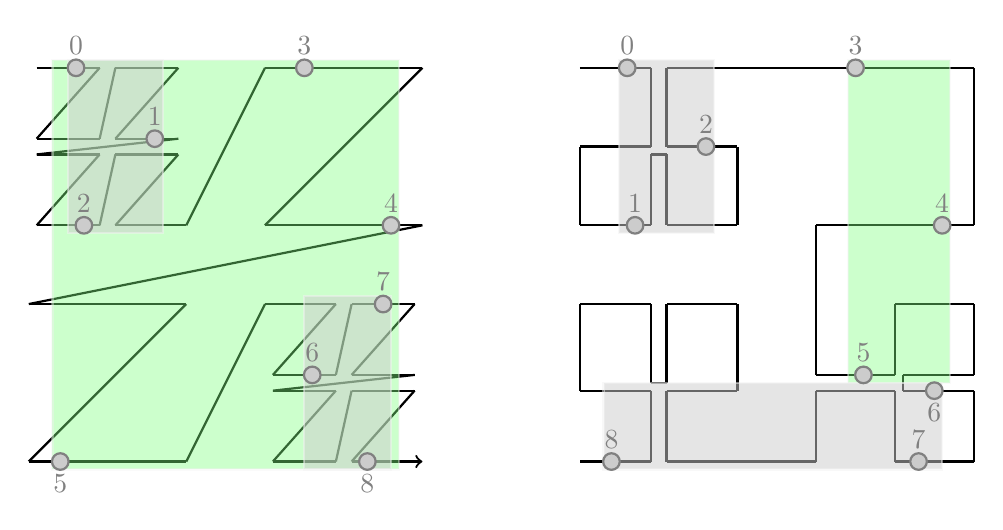
\begin{tikzpicture}[thick]
%\draw[black!50,fill=black!30] (2,2) circle (5pt);
% Morton
\draw[-] (.1,5) -- (.9,5);
\draw[-] (.9,5) -- (.1,4.1);
\draw[-] (.1,4.1) -- (.9,4.1);
\draw[-] (.9,4.1) -- (1.1,5);
\draw[-] (1.1,5) -- (1.9,5);
\draw[-] (1.9,5) -- (1.1,4.1);
\draw[-] (1.1,4.1) -- (1.9,4.1);
\draw[-] (1.9,4.1) -- (0.1,3.9);
\draw[-] (.1,3.9) -- (.9,3.9);
\draw[-] (.9,3.9) -- (.1,3);
\draw[-] (.1,3) -- (.9,3);
\draw[-] (.9,3) -- (1.1,3.9);
\draw[-] (1.1,3.9) -- (1.9,3.9);
\draw[-] (1.9,3.9) -- (1.1,3);
\draw[-] (1.1,3) -- (2,3);

\draw[-] (2,3) -- (3,5);
\draw[-] (3,5) -- (5,5);
\draw[-] (5,5) -- (3,3);
\draw[-] (3,3) -- (5,3);
\draw[-] (5,3) -- (0,2);
\draw[-] (0,2) -- (2,2);
\draw[-] (2,2) -- (0,0);
\draw[-] (0,0) -- (2,0);
\draw[-] (2,0) -- (3,2);

\draw[-] (3,2) -- (3.9,2);
\draw[-] (3.9,2) -- (3.1,1.1);
\draw[-] (3.1,1.1) -- (3.9,1.1);
\draw[-] (3.9,1.1) -- (4.1,2);
\draw[-] (4.1,2) -- (4.9,2);
\draw[-] (4.9,2) -- (4.1,1.1);
\draw[-] (4.1,1.1) -- (4.9,1.1);
\draw[-] (4.9,1.1) -- (3.1,.9);
\draw[-] (3.1,.9) -- (3.9,.9);
\draw[-] (3.9,.9) -- (3.1,0);
\draw[-] (3.1,0) -- (3.9,0);
\draw[-] (3.9,0) -- (4.1,0.9);
\draw[-] (4.1,0.9) -- (4.9,0.9);
\draw[-] (4.9,0.9) -- (4.1,0);
\draw[->] (4.1,0) -- (5,0);

% Hilbert
\draw[-] (7,5) -- (7.9,5);
\draw[-] (7.9,5) -- (7.9,4);
\draw[-] (7.9,4) -- (7,4);
\draw[-] (7,4) -- (7,3);
\draw[-] (7,3) -- (7.9,3);
\draw[-] (7.9,3) -- (7.9,3.9);
\draw[-] (7.9,3.9) -- (8.1,3.9);
\draw[-] (8.1,3.9) -- (8.1,3);
\draw[-] (8.1,3) -- (9,3);
\draw[-] (9,3) -- (9,4);
\draw[-] (9,4) -- (8.1,4);
\draw[-] (8.1,4) -- (8.1,5);
\draw[-] (8.1,5) -- (9,5);

\draw[-] (9,5) -- (10,5);
\draw[-] (10,5) -- (12,5);
\draw[-] (12,5) -- (12,3);
\draw[-] (12,3) -- (10,3);
\draw[-] (10,3) -- (10,2);

\draw[-] (10,2) -- (10,1.1);
\draw[-] (10,1.1) -- (11,1.1);
\draw[-] (11,1.1) -- (11,2);
\draw[-] (11,2) -- (12,2);
\draw[-] (12,2) -- (12,1.1);
\draw[-] (12,1.1) -- (11.1,1.1);
\draw[-] (11.1,1.1) -- (11.1,.9);
\draw[-] (11.1,.9) -- (12,.9);
\draw[-] (12,.9) -- (12,0);
\draw[-] (12,0) -- (11,0);
\draw[-] (11,0) -- (11,.9);
\draw[-] (11,.9) -- (10,.9);
\draw[-] (10,.9) -- (10,0);
\draw[-] (10,0) -- (9,0);

\draw[-] (9,0) -- (8.1,0);
\draw[-] (8.1,0) -- (8.1,.9);
\draw[-] (8.1,.9) -- (9,.9);
\draw[-] (9,.9) -- (9,2);
\draw[-] (9,2) -- (8.1,2);
\draw[-] (8.1,2) -- (8.1,1);
\draw[-] (8.1,1) -- (7.9,1);
\draw[-] (7.9,1) -- (7.9,2);
\draw[-] (7.9,2) -- (7,2);
\draw[-] (7,2) -- (7,.9);
\draw[-] (7,.9) -- (7.9,.9);
\draw[-] (7.9,.9) -- (7.9,0);
\draw[-] (7.9,0) -- (7,0);

% Add the particles over it 
\draw[black!5,opacity=.4,fill=green!50] (.3,-.1) rectangle (4.7,5.1);
\draw[black!5,opacity=0.5,fill=black!20] (.5,2.9) rectangle (1.7,5.1);
\draw[black!5,opacity=0.5,fill=black!20] (3.5,-0.1) rectangle (4.6,2.1);
% P1
\draw[black!50,fill=black!20] (0.6,5) circle (3pt) node[yshift=1pt,above] {0};
\draw[black!50,fill=black!20] (1.6,4.1) circle (3pt) node[yshift=1pt,above] {1};
\draw[black!50,fill=black!20] (.7,3) circle (3pt) node[yshift=1pt,above] {2};
% rect 1 
\draw[black!50,fill=black!20] (3.5,5) circle (3pt) node[yshift=1pt,above] {3};
\draw[black!50,fill=black!20] (4.6,3) circle (3pt) node[yshift=1pt,above] {4};
\draw[black!50,fill=black!20] (.4,0) circle (3pt) node[yshift=-1pt,below] {5};
% rect 1 
\draw[black!50,fill=black!20] (3.6,1.1) circle (3pt) node[yshift=1pt,above] {6};
\draw[black!50,fill=black!20] (4.5,2) circle (3pt) node[yshift=1pt,above] {7};
\draw[black!50,fill=black!20] (4.3,0) circle (3pt) node[yshift=-1pt,below] {8};
% rect 1 


% hilbert rectangles 
\draw[black!5,opacity=.4,fill=green!50] (10.4,1) rectangle (11.7,5.1);
\draw[black!5,opacity=0.5,fill=black!20] (7.5,2.9) rectangle (8.7,5.1);
\draw[black!5,opacity=0.5,fill=black!20] (7.3,-.1) rectangle (11.6,1);

% Hilbert particles
\draw[black!50,fill=black!20] (7.6,5) circle (3pt) node[yshift=1pt,above] {0};
\draw[black!50,fill=black!20] (7.7,3) circle (3pt) node[yshift=1pt,above] {1};
\draw[black!50,fill=black!20] (8.6,4) circle (3pt) node[yshift=1pt,above] {2};

\draw[black!50,fill=black!20] (10.5,5) circle (3pt) node[yshift=1pt,above] {3};
\draw[black!50,fill=black!20] (11.6,3) circle (3pt) node[yshift=1pt,above] {4};
\draw[black!50,fill=black!20] (10.6,1.1) circle (3pt) node[yshift=1pt,above] {5};

\draw[black!50,fill=black!20] (11.5,.9) circle (3pt) node[yshift=-1pt,below] {6};
\draw[black!50,fill=black!20] (11.3,0) circle (3pt) node[yshift=1pt,above] {7};
\draw[black!50,fill=black!20] (7.4,0) circle (3pt) node[yshift=1pt,above] {8};



\end{tikzpicture}